\chapter{Backpropagation}
\cite{chapter2}

%%
\section{定义}
$b^l_j$ : $l^{\rm th}$ 层 $j^{\rm th}$ neuron 的偏置bias. \par
$a^l_j$ : $l^{\rm th}$ 层 $j^{\rm th}$ neuron 的激活activation.

$w^l_{jk}$ : $l^{th}$层的 node 的权重,
$l^{\rm th}$ 层的 $j^{\rm th}$ neuron \textcolor{red}{$\Lleftarrow$}
$(l-1)^{\rm th}$ 层的$k^{\rm th}$ neuron
%\tikz \fill (0,0) circle(2ex);
如图:\par
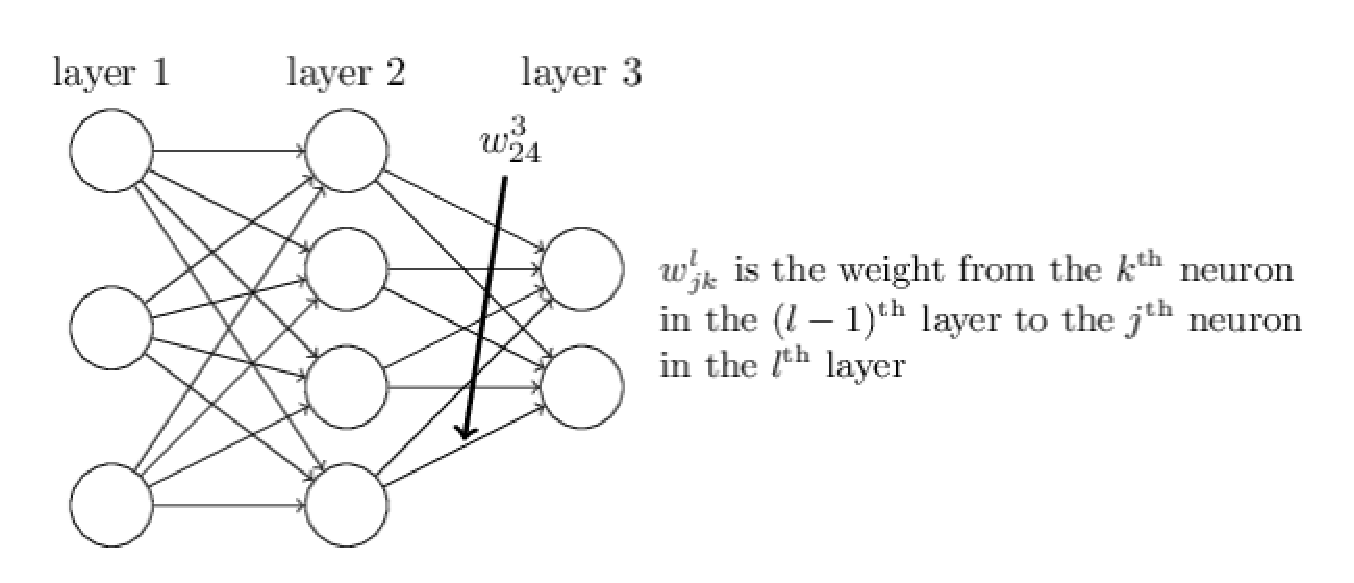
\includegraphics[scale=0.5]{fig/weight_definition.eps}

\centerline {$a^{l}_j = \sigma\left(\sum_k w^{l}_{jk} a^{l-­1}_k + b^l_j \right)$}
向量表示:\par
\centerline{$a^{l} =\sigma(w^l a^{l-­1}+b^l)$}
矩阵表示:
\begin{center}
$a^l = \sigma(z^l)$\\
$z^l \equiv w^l a^{l-­1}+b^l$
\end{center}
其中:\par
\centerline{$z^l_j = \sum_k w^l_{jk} a^{l­-1}_k+b^l_j$}

\section{cost function的两个假设}
后向传播的目的是得到代价函数$C$对于网络中任意权重$w$或偏差$b$的偏导数:\par
\centerline{$\frac {\partial C}{\partial w}$ 和 $\frac{\partial C}{\partial b}$}

二次代价函数的形式:\par
\centerline{$C=\frac{1}{2n}\sum_x \|y(x)-­a^L(x)\|^2$}\par
\noindent$n$为样本数;$y=y(x)$为$x$对应的期望输出;$L$为网络层数;
$a^L=a^L(x)$是输入为$x$时的网络激活输出向量。

关于代价函数,什么样的假设可以使得后向传播能够应用起来?\par
\textcolor{red}{第一个假设}是代价函数能够被写成基于每一个独立的训练样本$x$求代价函数$C_x$的平均值:
$C_x=\frac{1}{n}\sum_x C_x$。二次代价函数满足此条件,其中每一个样本的代价为:
$C_x = \frac{1}{2} \|y­-a^L\|^2$ \par
需要这个假设的原因是因为后向传播实际上让我们能够基于每一个样本计算偏导数
$\partial C_x / \partial w$ 和 $\partial C_x / \partial b$
我们然后在整个选练样本基础上经过平均而求出
$\partial C / \partial w$ 和 $\partial C / \partial b$。

\textcolor{red}{第二个}关于代价函数的假设是可以把它当作神经网路激活输出的一个函数,
$cost \ C = C(a^L)$
二次型代价函数满足这个假定,因为对于每一个样本$x$,代价函数可以写成:\par
\centerline{$C = \frac{1}{2} \|y-­a^L\|^2 = \frac{1}{2} \sum_j (y_j-a^L_j)^2$}

Hadamard乘积或Schur乘积,$\odot$,即逐元素相乘

\section{backpropagation背后的基础四等式}
引入中间变量$\delta^l_j$,为做网络中第$l^{\rm th}$层第$j^{\rm th}$神经元的误差:
$\delta^l_j \equiv \frac{\partial C}{\partial z^l_j}$

\subsection{输出层的误差等式:}
\begin{align} 
\delta^L_j = \frac{\partial C}{\partial a^L_j} \sigma'(z^L_j). \tag{BP1}
\end{align}\par
矩阵形式:
\begin{align}
\delta^L = \nabla_a C \odot \sigma'(z^L). \tag{BP1a}\
\end{align}

\subsection{误差$\delta^l$用下一层的误差$\delta^{l+1}$表示:}
\begin{align}
\delta^l = ((w^{l+1})^T \delta^{l+1}) \odot \sigma'(z^l), \tag{BP2}
\end{align}

\subsection{代价函数相对网络中任意偏置变化率的等式:}
\begin{align}
\frac{\partial C}{\partial b^l_j} = \delta^l_j. \tag{BP3}
\end{align}
误差$\delta^l_j$和变化率$\partial C / \partial b^l_j$精确相同,简短形式为:
\begin{align}
\frac{\partial C}{\partial b} = \delta,\tag{31}
\end{align}

\subsection{代价函数相对网络中任意权重变化率的等式:}
\begin{align}
\frac{\partial C}{\partial w^l_{jk}} = a^{l-­1}_k \delta^l_j. \tag{BP4}
\end{align}
改写为:
\begin{align}
\frac{\partial C}{\partial w} = a_{\rm in} \delta_{\rm out}, \tag{32}
\end{align}
可以看到,(BP4) 的结果就是小的激活神经元的权重会比较缓慢的学习。

%%%%%%%%%%%%%%%
\begin{framed}
summary: backpropagation 方程
\begin{align*}
\delta^L & = \nabla_a C \odot \sigma'(z^L). \tag{BP1} \\
\delta^l & = ((w^{l+1})^T \delta^{l+1}) \odot \sigma'(z^l), \tag{BP2} \\
\frac{\partial C}{\partial b^l_j} & = \delta^l_j. \tag{BP3} \\
\frac{\partial C}{\partial w^l_{jk}} & = a^{l-­1}_k \delta^l_j. \tag{BP4}
\end{align*}
矩阵形式:

(BP1)重写为
\begin{align}
\delta^L = \Sigma'(z^L) \nabla_a C,\tag{1}
\end{align}
其中,$\Sigma'(z^L)$是一个对角线元素为$\sigma'(z^L_j)$的方阵,且其非对角线元素都是零。
此矩阵与$\nabla_a C$进行传统的矩阵乘法

(BP2)重写为:
\begin{align}
\delta^l = \Sigma'(z^l) (w^{l+1})^T\delta^{l+1} \tag{2}
\end{align}

合并(1)和(2)可得:
\begin{align}
\delta^l = \Sigma'(z^l)(w^{l+1})^T \ldots 
\Sigma'(z^{L-­1}) (w^L)^T \Sigma'(z^L) \nabla_a C \tag{3}
\end{align}
\end{framed}

\section{The Backpropagation}
\begin{framed}
\textbf{1. Input $x$:} \par \indent \indent \indent 
Set the corresponding activation $a^{1}$ for the input layer.

\textbf{2. Feedforward:} \par \indent \indent \indent 
For each $l = 2, 3, \ldots, L$ compute \par
\centerline{$z^{l} = w^l a^{l-­1}+b^l$ and $a^{l} = \sigma(z^{l})$.}

\textbf{3. Output error $\delta^L$:} \par \indent \indent \indent 
Compute the vector 
\[ \delta^{L} = \nabla_a C \odot \sigma'(z^L) . \]

\textbf{4. Backpropagate the error:} \par \indent \indent \indent 
For each $l = L-1,L-­2,\ldots, 2$ \ compute 
\[ \delta^{l} = ((w^{l+1})^T \delta^{l+1}) \odot \sigma'(z^{l}).\] \par

\textbf{5. Output: The gradient of the cost function}\par 
\centerline{$\frac{\partial C}{\partial w^l_{jk}} = 
a^{l-­1}_k \delta^l_j$ and $\frac{\partial C}{\partial b^l_j} = \delta^l_j$.}
\end{framed}

单个样本训练过程:
\begin{framed}
1. 输入训练样本集合 

2. 对于每一个训练样本$x$: \par
\indent \indent 设置对应的输入激活 $a^{x,1}$执行以下步骤:\par
\indent \indent $\circ$向前:对于每一层$l = 2, 3, \ldots, L$,计算 \par
\centerline{$z^{x,l} =w^l a^{x,l-­1}+b^l$ 和 $a^{x,l} = \sigma(z^{x,l})$}
\indent \indent $\circ$输出层误差$\delta^{x,L}$:计算向量
\[ \delta^{x,L} = \nabla_a C_x \odot \sigma'(z^{x,L}).\] 
\indent \indent $\circ$后向传播误差:对于每一层$l = L-­1,L-­2,\ldots, 2$,计算
\[ \delta^{x,l} = ((w^{l+1})^T \delta^{x,l+1}) \odot \sigma'(z^{x,l}).\]

3. 梯度下降:按下面规则更新,\par
\begin{align}
w_k & \longrightarrow w'_k = w_k - \eta \frac{\partial C_x}{\partial w_k} \\
b_l & \longrightarrow b'_l = b_l - \eta \frac{\partial C_x}{\partial b_l}
\end{align}
即,对于每一层$l = L, L-­1, \ldots, 2$,更新为: \par
\begin{align}
w^l & \rightarrow w^l­ -\frac{\eta}{m} \sum_x\delta^{x,l} (a^{x,l-­1})^T,\\ 
b^l & \rightarrow b^l­ -\frac{\eta}{m} \sum_x \delta^{x,l}
\end{align}
\end{framed}
%\cite{hu_improved_2015}

